\documentclass[a4paper,12pt]{article}
\usepackage[brazil]{babel}
\usepackage[utf8]{inputenc}
\usepackage[T1]{fontenc}
\usepackage{geometry}
\usepackage{setspace}
\usepackage{titlesec}
\usepackage{hyperref}
\usepackage{graphicx}
\usepackage{caption}
\usepackage{subcaption}
\usepackage{fancyhdr}
\usepackage{xcolor}

%%%%%%%%%%%%%%%%%%%%%%%%%%%%%%%%%%%%%%%%%%%%%%%%%%
% These are some new commands that may be useful 
% for paper writing in general. If other new commands
% are needed for your specific paper, please feel 
% free to add here. 
%
% The currently available commands are organized in: 
% 1) Systems
% 2) Quantities
% 3) Energies and units
% 4) particle species
% 5) Colors package
% 6) hyperlink
%%%%%%%%%%%%%%%%%%%%%%%%%%%%%%%%%%%%%%%%%%%%%%%%%%

\usepackage{amsmath}
\usepackage{amssymb}
\usepackage{upgreek}
\usepackage{multirow}
\usepackage{setspace}% http://ctan.org/pkg/setspace
\usepackage{fancyhdr}
\usepackage{datetime}

% 1) SYSTEMS
\newcommand{\btc}               {\textbf{BTC}}
\newcommand{\btcspace}          {\textbf{BTC} }
\newcommand{\pow}               {\textbf{PoW}}

% 4) definition to references, biblatex and hyperlink
\usepackage[backend=bibtex, 
style=nature,  %style reference.
sorting=none,
firstinits=true %first name abbreviate
]{biblatex}

\usepackage{hyperref}
\hypersetup{
    colorlinks=true, %set "true" if you want colored links
    linktoc=all,     %set to "all" if you want both sections and subsections linked
    linkcolor=blue,  %choose some color if you want links to stand out
    citecolor= blue, % color of \cite{} in the text.
    urlcolor  = blue, % color of the link for the paper in references.
}

% 5) Tikz and figures
\usepackage{epsfig}
\usepackage{lmodern}
\usepackage{mathtools}
\usepackage[utf8]{luainputenc}
\usepackage{xspace}
\usepackage{tikz}
\usepackage{pgfplots}
\pgfplotsset{compat=newest}

\usetikzlibrary{positioning}
\usepackage{subcaption}

% 6) colors:
\usepackage{xcolor}
\definecolor{ao(english)}{rgb}{0.0, 0.5, 0.0} % dark green

% 7) Add lines numbers
%\usepackage{lineno}

% add pdf file to thesis:
\usepackage{pdfpages}

\usepackage[most]{tcolorbox}

%textmarker style from colorbox doc
\tcbset{textmarker/.style={%
        enhanced,
        parbox=false,boxrule=0mm,boxsep=0mm,arc=0mm,
        outer arc=0mm,left=6mm,right=3mm,top=7pt,bottom=7pt,
        toptitle=1mm,bottomtitle=1mm,oversize}}


% define new colorboxes
\newtcolorbox{hintBox}{textmarker,
    borderline west={6pt}{0pt}{yellow},
    colback=yellow!10!white}
\newtcolorbox{importantBox}{textmarker,
    borderline west={6pt}{0pt}{red},
    colback=red!10!white}
\newtcolorbox{noteBox}{textmarker,
    borderline west={6pt}{0pt}{green},
    colback=green!10!white}

% define commands for easy access
\newcommand{\note}[1]{\begin{noteBox} \textbf{} #1 \end{noteBox}}
\newcommand{\warning}[1]{\begin{hintBox} \textbf{Warning:} #1 \end{hintBox}}
\newcommand{\important}[1]{\begin{importantBox} \textbf{} #1 \end{importantBox}}

\hypersetup{
    colorlinks=true,% make the links colored
    linkcolor=blue
}

\usepackage{setspace}
\addbibresource{bibliography.bib}

\newcommand{\printingbibliography}{%

    \pagestyle{myheadings}
    \markright{}
    \sloppy
    \printbibliography[heading=bibintoc, % add to table of contents
                   title=Refer\^encias % Chapter name
                  ]
    \fussy%
}
\PassOptionsToPackage{table}{xcolor}
\renewcommand{\baselinestretch}{1.5}

\pagestyle{fancy}
\fancyhf{}
\renewcommand{\headrulewidth}{0pt}
\fancyhead[R]{\thepage}

\geometry{a4paper,top=30mm,bottom=20mm,left=30mm,right=20mm}

\titleformat*{\section}{\bfseries\large}
\titleformat*{\subsection}{\bfseries\normalsize}

\title{ \textbf{\href{https://www.curso-objetivo.br/vestibular/resolucao-comentada/fuvest/simulado-2026/prova-s1-simulado-fuvest-2026.pdf}{Simulado Prova de Conhecimentos Gerais FUVEST 2026 – Prova S1}} \\
}
\author{Andr\'e V. Silva}
\date{\today}

\begin{document}

\maketitle

\begin{figure}[h!]
    \centering
    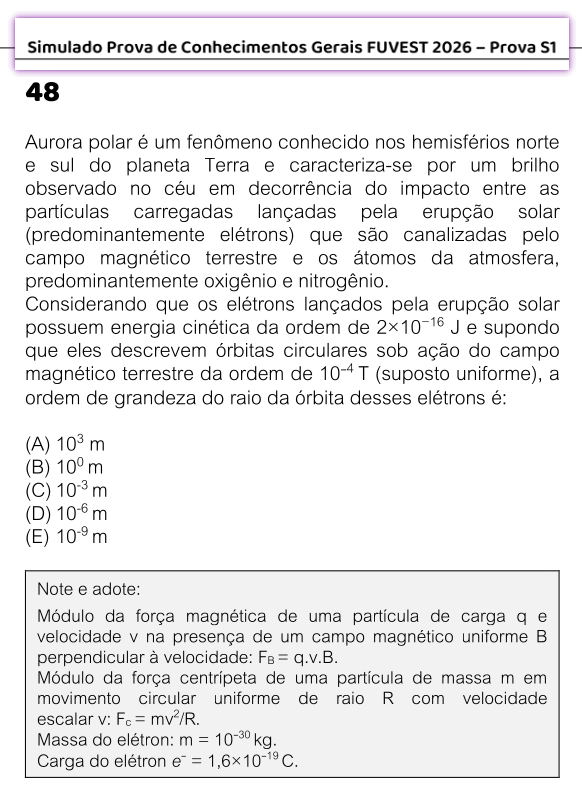
\includegraphics[width=0.7\textwidth]{images/q48.png}
    \caption{}
    \label{fig:trajetoria}
\end{figure}

\subsection*{Resolução}



A força magnética atua como força centrípeta:

\[
qvB = \frac{mv^2}{R}
\]

Simplificando:

\[
R = \frac{mv}{qB}
\]

Da energia cinética:

\[
E_c = \frac{1}{2}mv^2
\Rightarrow
v = \sqrt{\frac{2E_c}{m}}
\]

Substituindo:

\[
v = \sqrt{\frac{2 \cdot 2 \times 10^{-16}}{10^{-30}}}
= 2 \times 10^7 \, \text{m/s}
\]

Raio:

\[
R = \frac{10^{-30} \cdot 2 \times 10^7}{1{,}6 \times 10^{-19} \cdot 10^{-4}}
\approx 1{,}25 \, \text{m}
\]

Ordem de grandeza:

\[
R \sim 10^0 \, \text{m}
\]

\vspace{0.5cm}

\textcolor{red}{\textbf{Solução:}}\\
A resposta correta é \colorbox{green!50}{\textbf{(B)}}.

\newpage

\begin{figure}[h!]
    \centering
    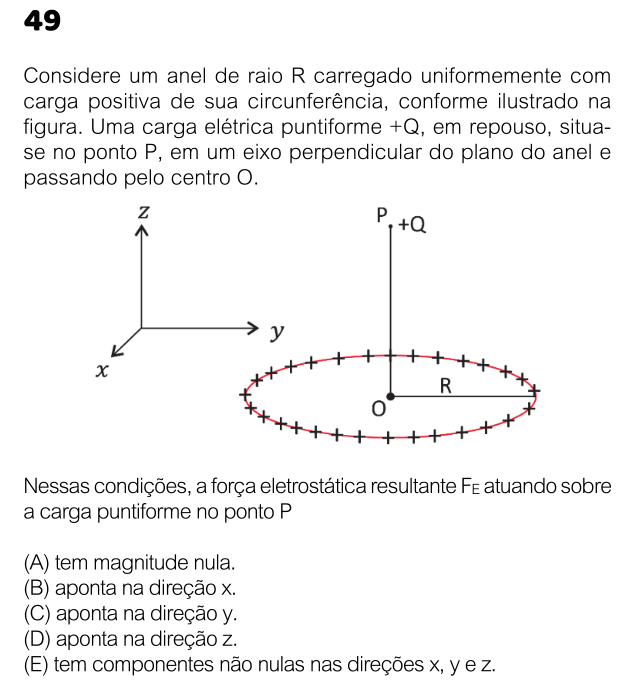
\includegraphics[width=0.9\textwidth]{images/q49.png}
    \caption{}
    \label{fig:trajetoria}
\end{figure}

\subsection*{Resolução}

\textbf{1. Simetria do problema}

O anel possui distribuição \textbf{uniforme} de carga. Isso implica que:

\begin{itemize}
\item Para cada elemento de carga $dq$ em uma posição do anel, existe outro elemento diametralmente oposto.
\item As componentes do campo elétrico no plano do anel (direções $x$ e $y$) se cancelam mutuamente.
\end{itemize}

\textbf{Conclusão parcial:}  
As componentes $E_x$ e $E_y$ são nulas:
\[
E_x = 0 \quad \text{e} \quad E_y = 0
\]

\textbf{2. Componente ao longo do eixo $z$}

Considere um elemento de carga $dq$ no anel. O campo elétrico produzido por esse elemento no ponto $P$ tem direção ao longo da linha que liga $dq$ a $P$.

Decompondo esse campo:

\begin{itemize}
\item A componente perpendicular ao eixo $z$ é cancelada por simetria.
\item A componente ao longo do eixo $z$ é somada para todos os elementos.
\end{itemize}

Logo, o campo elétrico resultante no ponto $P$ aponta exclusivamente na direção do eixo $z$.

\textbf{3. Sentido do campo elétrico}

Como:

\begin{itemize}
\item o anel está carregado positivamente,
\item a carga $+Q$ também é positiva,
\end{itemize}

o campo elétrico produzido pelo anel no ponto $P$ aponta \textbf{para fora do anel}, isto é, no sentido positivo do eixo $z$.

\textbf{4. Força elétrica}

A força sobre a carga $+Q$ é dada por:

\[
\vec{F}_E = Q \vec{E}
\]

Como $Q > 0$, a força tem a \textbf{mesma direção e sentido} do campo elétrico.

\textbf{Conclusão final:}

\begin{itemize}
\item A força não possui componentes em $x$ ou $y$.
\item A força aponta ao longo do eixo $z$.
\end{itemize}

\vspace{0.5cm}

\textcolor{red}{\textbf{Resposta:}}\\

A resposta correta é alternativa \colorbox{green!50}{\textbf{(D)}}.

\newpage

\begin{figure}[h!]
    \centering
    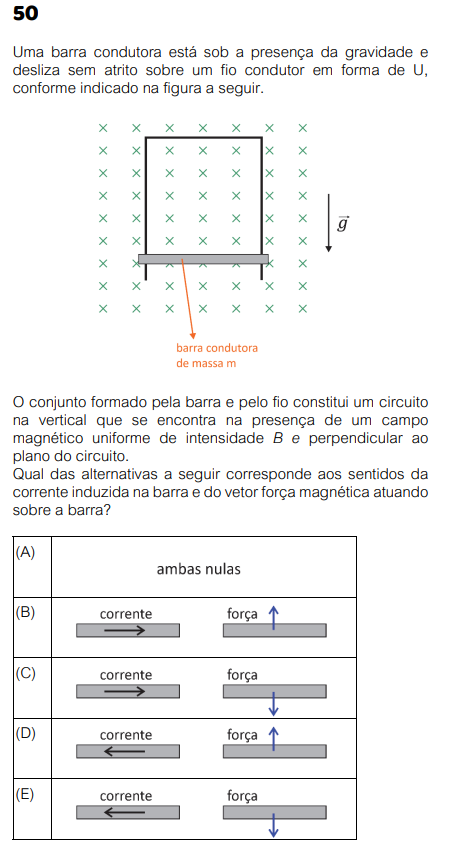
\includegraphics[width=0.8\textwidth]{images/q50.png}
    \caption{}
    \label{fig:trajetoria}
\end{figure}


\subsection*{Solu\c{c}\~ao}

\textbf{1. Análise do movimento}

A barra está sob a ação da gravidade, portanto ela tende a se mover \textbf{para baixo}.

\textbf{2. Variação do fluxo magnético}

O fluxo magnético é dado por:

\[
\Phi_B = B \cdot A
\]

Como a barra desce, a área do circuito \textbf{aumenta}, logo:

\[
\frac{d\Phi_B}{dt} > 0
\]

Ou seja, o fluxo magnético \textbf{entrando no plano} está aumentando.

\textbf{3. Lei de Lenz}

Pela Lei de Lenz:

\begin{quote}
A corrente induzida surge de modo a \textbf{opor-se à variação do fluxo magnético}.
\end{quote}

Como o fluxo entrando no plano está aumentando, a corrente induzida deve criar um campo magnético \textbf{saindo do plano}.

\textbf{4. Regra da mão direita}

Para gerar um campo magnético saindo do plano:

\begin{itemize}
\item A corrente deve circular no sentido \textbf{anti-horário}.
\end{itemize}

Logo, na barra (parte inferior do circuito):

\[
\text{corrente da esquerda para a direita}
\]

\textbf{5. Força magnética na barra}

A força magnética é dada por:

\[
\vec{F} = i \vec{L} \times \vec{B}
\]

Aplicando a regra da mão direita:

\begin{itemize}
\item Corrente: da esquerda para a direita
\item Campo magnético: entrando no plano
\end{itemize}

Resulta:

\[
\vec{F} \text{ aponta para cima}
\]

\textbf{6. Interpretação física}

A força magnética:

\begin{itemize}
\item é contrária ao movimento da barra,
\item atua como uma força de resistência (consistente com a Lei de Lenz).
\end{itemize}

\vspace{0.5cm}

\textcolor{red}{\textbf{Solu\c{c}\~ao:}}\\

A resposta correta é alternativa \colorbox{green!50}{\textbf{(B)}}.

\newpage

\begin{figure}[h!]
    \centering
    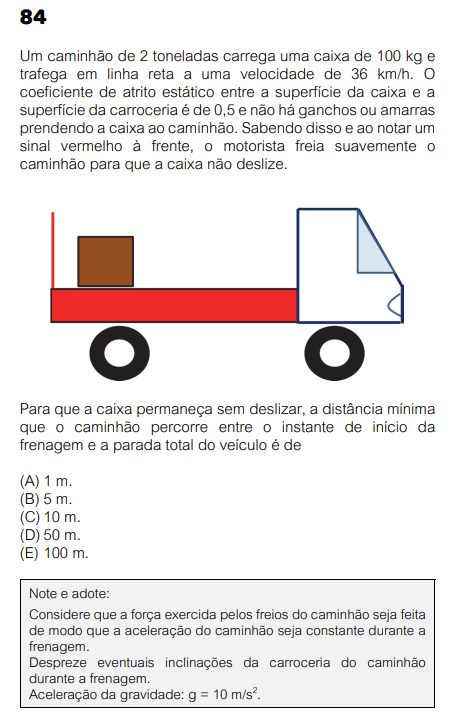
\includegraphics[width=0.87\textwidth]{images/q84.png}
    \caption{}
    \label{fig:trajetoria}
\end{figure}

\newpage

\textcolor{red}{\textbf{Solução:}}\\

\textbf{1. Conversão da velocidade:}

\[
v_0 = 36\ \text{km/h} = 10\ \text{m/s}
\]

\textbf{2. Condição para não haver deslizamento:}

A força de atrito estático máxima é responsável por desacelerar a caixa:

\[
f_{\text{máx}} = \mu_e N = \mu_e m g
\]

Pela segunda lei de Newton:

\[
f = m a
\]

Logo, a desaceleração máxima sem deslizamento é:

\[
a_{\text{máx}} = \mu_e g
\]

Substituindo os valores:

\[
a_{\text{máx}} = 0{,}5 \cdot 10 = 5\ \text{m/s}^2
\]

\textbf{3. Cálculo da distância mínima de frenagem:}

Utilizamos a equação de Torricelli:

\[
v^2 = v_0^2 + 2 a \Delta s
\]

Como o caminhão para, $v = 0$:

\[
0 = (10)^2 - 2 \cdot 5 \cdot \Delta s
\]

\[
0 = 100 - 10 \Delta s
\]

\[
\Delta s = 10\ \text{m}
\]

\textbf{4. Conclusão:}

A menor distância possível para que a caixa não deslize ocorre quando a desaceleração é máxima (igual à fornecida pelo atrito estático).

\vspace{0.5cm}

A resposta correta é alternativa \colorbox{green!50}{\textbf{(C) 10 m}}.

\newpage

\begin{figure}[h!]
    \centering
    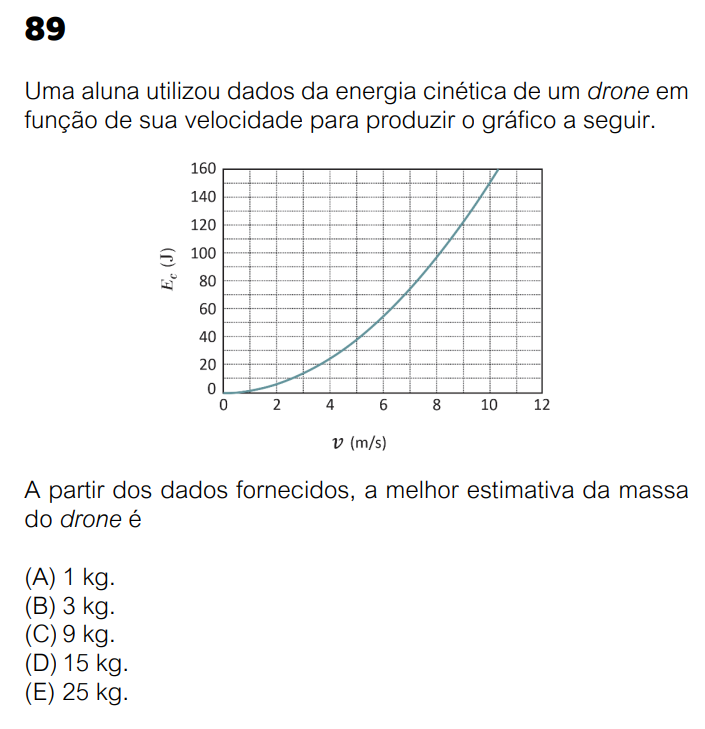
\includegraphics[width=0.87\textwidth]{images/q89.png}
    \caption{}
    \label{fig:trajetoria}
\end{figure}


\textcolor{red}{\textbf{Solu\c{c}\~ao:}}\\

\textbf{1. Rela\c{c}\~ao f\'isica fundamental:}

A energia cin\'etica \'e dada por:

\[
E_c = \frac{1}{2} m v^2
\]

\textbf{2. Extra\c{c}\~ao de um ponto do gr\'afico:}

Observando o gr\'afico, para:

\[
v = 10\ \text{m/s}, \quad E_c \approx 150\ \text{J}
\]

\textbf{3. Substitui\c{c}\~ao na f\'ormula:}

\[
150 = \frac{1}{2} m (10)^2
\]

\[
150 = \frac{1}{2} m \cdot 100
\]

\[
150 = 50m
\]

\textbf{4. Determina\c{c}\~ao da massa:}

\[
m = \frac{150}{50} = 3\ \text{kg}
\]

\textbf{5. Conclus\~ao:}

A massa do drone estimada a partir do gr\'afico \'e:

\vspace{0.5cm}

A resposta correta \'e alternativa \colorbox{green!50}{\textbf{(B) 3 kg}}.


\newpage

\begin{figure}[h!]
    \centering
    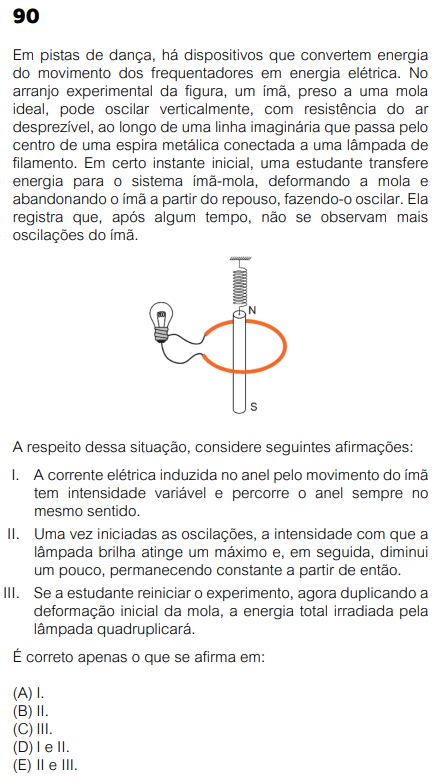
\includegraphics[width=0.8\textwidth]{images/q90.png}
    \caption{}
    \label{fig:trajetoria}
\end{figure}

\newpage

\subsection*{Indu\c{c}\~ao Eletromagn\'etica e Dissipa\c{c}\~ao de Energia}

Em pistas de dan\c{c}a modernas, dispositivos podem converter energia mec\^anica em energia el\'etrica. Em um arranjo experimental, um \'im\~a est\'a preso a uma mola ideal e pode oscilar verticalmente ao longo do eixo de uma espira met\'alica ligada a uma l\^ampada de filamento. 

Inicialmente, uma estudante deforma a mola e solta o sistema a partir do repouso, fazendo o \'im\~a oscilar. Ap\'os certo tempo, observa-se que o movimento cessa completamente.

\textbf{Com base nessa situa\c{c}\~ao, responda:}

\begin{itemize}
\item[(a)] Explique, com base na Lei de Faraday e na Lei de Lenz, como surge a corrente el\'etrica induzida na espira durante o movimento do \'im\~a e justifique por que o sentido dessa corrente se altera ao longo do tempo.

\item[(b)] Descreva o comportamento da intensidade da corrente el\'etrica e do brilho da l\^ampada ao longo do tempo, relacionando com a varia\c{c}\~ao da energia mec\^anica do sistema.

\item[(c)] Justifique por que as oscila\c{c}\~oes do sistema cessam, mesmo na aus\^encia de resist\^encia do ar.

\item[(d)] Sabendo que a energia potencial el\'astica inicial \'e dada por $E = \frac{1}{2}kx^2$, analise o que ocorre com a energia total dissipada na l\^ampada se a deforma\c{c}\~ao inicial da mola for duplicada. Apresente a rela\c{c}\~ao matem\'atica envolvida.

\end{itemize}

\vspace{0.5cm}

\textcolor{red}{\textbf{Solu\c{c}\~ao Esperada:}}\\

\textbf{(a)} A varia\c{c}\~ao do fluxo magn\'etico atrav\'es da espira, causada pelo movimento do \'im\~a, induz uma for\c{c}a eletromotriz segundo a Lei de Faraday. Pela Lei de Lenz, a corrente induzida tem sentido tal que se op\~oe \`a varia\c{c}\~ao do fluxo, o que implica invers\~ao do sentido da corrente quando o \'im\~a se aproxima ou se afasta da espira.

\textbf{(b)} A corrente induzida possui intensidade vari\'avel, sendo maior quando a velocidade do \'im\~a \'e maior. Como a energia mec\^anica do sistema diminui ao longo do tempo, a intensidade da corrente tamb\'em diminui, resultando em um brilho progressivamente menor da l\^ampada, at\'e se apagar.

\textbf{(c)} As oscila\c{c}\~oes cessam porque h\'a convers\~ao de energia mec\^anica em energia el\'etrica, dissipada na l\^ampada (efeito Joule). Esse processo atua como uma for\c{c}a dissipativa eletromagn\'etica, amortecendo o movimento.

\textbf{(d)} Se a deforma\c{c}\~ao inicial for duplicada ($x \rightarrow 2x$), a energia inicial torna-se:

\[
E' = \frac{1}{2}k(2x)^2 = 4E
\]

Logo, a energia total dissipada na l\^ampada tamb\'em quadruplica.


%%%%%%%% Bibliography 
% Os comandos para incluir as referências bibliográficas
\printingbibliography

\end{document}
